\capitulo{3}{Conceptos teóricos}

Este punto nace ante la necesidad de enmarcar el proyecto dentro de las tecnologías y elementos que utilizaremos durante todo el proyecto y que no tienen por qué conocerse.

El término ‘domótica’ es el pilar principal del proyecto y, por ello, comenzaré explicando lo que es y como lo enfocaremos:

\section{Domótica}
La domótica podemos definirla como aquel conjunto de elementos capaces de automatizar una vivienda aportando un beneficio.
En nuestro caso, nuestro sistema domótico deberá controlar luces, persianas y calefacción permitiendo un aumento del confort y la seguridad, además de permitir un consumo eficiente de recursos a la hora de climatizar la vivienda.

\section{RaspberryPi}
En nuestro proyecto tendremos el control de la instalación domótica desde una Raspberry Pi. 
Para dar un enfoque muy general, podemos decir que las placas RaspberryPi son microordenadores que disponen de poca potencia si las comparamos con equipos usuales pero, disponen de suficiente potencia para llevar a cabo este tipo de proyectos.

Se diseñaron en su origen por la RaspBerry Pi Foundation en el Reino Unido para dotar de equipos informáticos a los centros de estudios a un bajo coste, pero el proyecto ha evolucionado para poder desarrollar, además, otras muchas tareas como puede ser nuestro caso, que la utilizaremos como ‘núcleo’ de toda nuestra instalación domótica y, será donde configuremos todo el entorno domótico de la vivienda.
Estas placas pueden ejecutar con agilidad distribuciones Linux y, desde sus distribuciones podemos interactuar con sus famosos “GPIO”.
\begin{center}
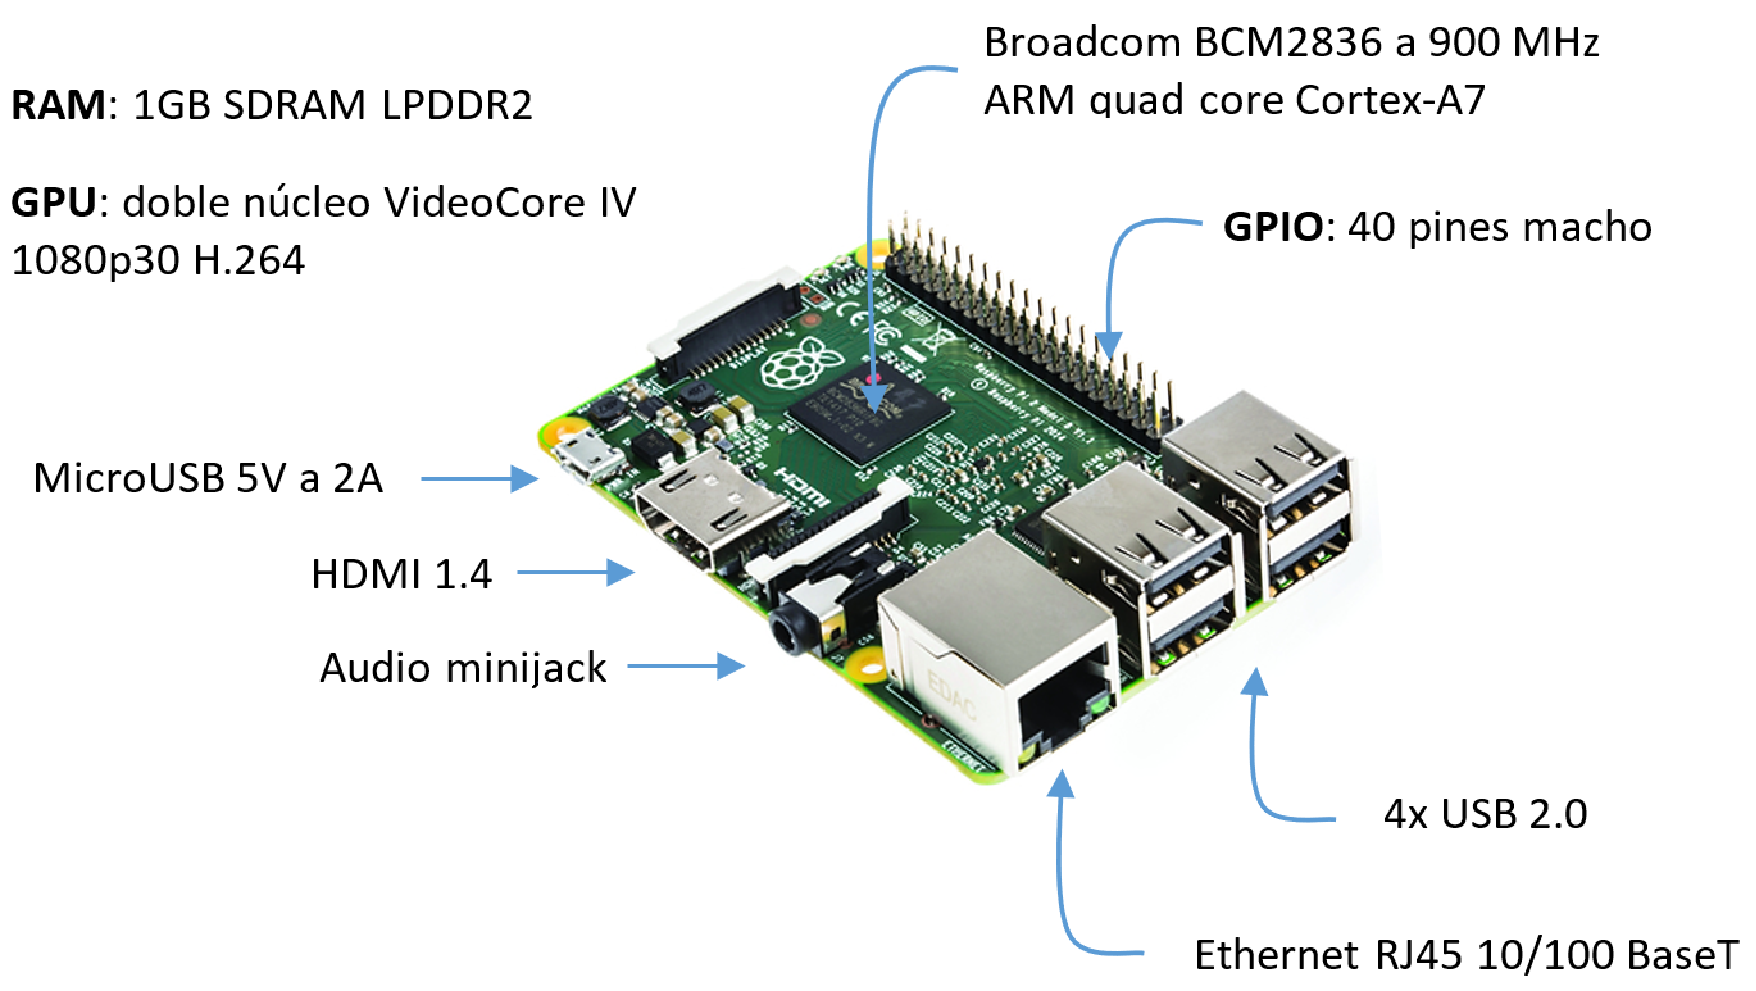
\includegraphics[width=\textwidth]{img/RBP2B.pdf}
\end{center}

\section{GPIO}
Éstos son unos puertos de entrada y salida conformados en forma de pines que están albergados en la placa, con los que enviaremos órdenes a otros dispositivos externos para que realicen las tareas que les designemos. En nuestro caso, servirán para controlar unos relés para conseguir una acción final.


\section{Relé}
Es un dispositivo electromagnético que desempeña la misma función de un interruptor, es decir, con nuestros relés, dejaremos pasar la energía eléctrica, o no, a nuestros dispositivos.

\section{Distribución Linux (Raspbian)}
Como he comentado anteriormente, pretendo correr una distribución Linux en nuestro microPc. Las placas Raspberry Pi disponen de unas distribuciones de Linux desarrolladas expresamente para su hardware desde la Raspberry Pi Foundation. De esta manera conseguimos que el entorno esté diseñado para el hardware donde será ejecutado incluyendo, además, utilidades preinstaladas para explotarlas más fácil y eficientemente.

\section{Funcionamiento autónomo}
Se pretende que tras pocas configuraciones el sistema sea capaz de funcionar extrayendo información de Internet y decidiendo que acción realizar en cada caso a partir de ese momento.

\section{Escalabilidad}
Como cualquier proyecto de calidad debe ser escalable, esto es, debe existir la posibilidad de que sea ampliado fácilmente.

\section{Acceso multiplataforma}
En este caso dispondremos de un acceso GUI\footnote{Traducción del inglés: 'Graphical User Interface'} (Interfaz gráfica) o CLI\footnote{Traducción del inglés: 'Command Line Interface'} (Línea de comandos) a nuestro equipo.

\section{Ahorro energético}
El ahorro energético se produce al permitir que la temperatura exterior incida, o no, en la vivienda para conseguir las condiciones deseadas optimizando el consumo de recursos.

\section{Web Scraping}
Es una técnica utilizada para extraer información de una página web utilizando las etiquetas de que dispone para movernos por los elementos de ésta.
En nuestro caso, podremos utilizarlo desde Python con beautifulsoup.

\section{API}
Es el acrónimo de ‘Application Programming Interfaces’ que, traducido al castellano significa ‘Interfaz de Programación de Aplicaciones’. Estas interfaces nos sirven información que podremos utilizar en un desarrollo.
Por ejemplo, para obtener la ubicación de la máquina Raspberry Pi accedemos a una API pública que nos devolverá información que podremos procesar a nuestro gusto.
Podemos acceder a esta \url{http://ip-api.com/json/?fields=country,regionName,city,lat,lon,isp,query}.
Y obtendremos los valores de país, región, ciudad, latitud, longitud, ISP y dirección IP.
Estos valores, podremos procesarlos desde Python como json.

\section{json}
Es el acrónimo en inglés de ‘JavaScript Object Notation’ y sirve para almacenar información de forma estructurada mediante etiquetas.

\section{RETB}
Es el acrónimo de Reglamento electrotécnico para baja tensión y en él se recoge la normativa eléctrica aplicable en domicilios.
Esta norma acaba de ser actualizada y podemos disponer de la información en páginas oficiales como puede ser el BOE\footnote{\url{https://www.boe.es/biblioteca_juridica/codigos/abrir_pdf.php?fich=326_Reglamento_electrotecnico_para_baja_tension_e_ITC.pdf}}.
Del documento ICT-BT-21\footnote{\url{http://eschoform.educarex.es/useruploads/r/c/886/scorm_imported/88234455166233572664/media/guia_bt_21.pdf}} podemos extraer información para realizar las instalaciones eléctricas de nuestro sistema domótico como el número máximo de cables a introducir por un tubo eléctrico.


\section{Normativa de ICT}
Como figura en el BOE 143, de 16 de junio de 2011: “El Reglamento regulador de las infraestructuras comunes de telecomunicaciones para el acceso a los servicios de telecomunicación en el interior de las edificaciones, aprobado por el Real Decreto 346/2011, de 11 de marzo.
Debemos regirnos por esta normativa a la hora de hacer cualquier instalación de comunicaciones nueva dentro de domicilios.
Podemos informarnos y ampliar información en la publicación del BOE\footnote{\url{https://www.boe.es/buscar/pdf/2011/BOE-A-2011-10457-consolidado.pdf}}.

Por otro lado, disponemos de guías para instaladores con dibujos y tablas que facilitan la comprensión, como puede ser la documentación que publica Televés\footnote{\url{https://docs.televes.com/web/Legislacion/m_ict2_3ed_reglamento_0.pdf}}

De este punto, obtendremos la norma para introducir cableado ICT conforme a norma.

Tras hacer un estudio en mi domicilio, no necesitaré utilizar la normativa de ICT porque toda la instalación se realizará mediante canales eléctricos, pero está bien conocer la norma para, en caso de necesitarla poder hacer uso de ella correctamente.

\section{Cableado estructurado}
El establecimiento de un sistema de cableado estructurado consiste en la organización de los cables en un recinto conforme a una norma y constituye el nivel básico de cualquier red de comunicaciones.
Al contar y cumplir con este estándar nos damos cuenta de que tendremos instalaciones limpias, uniformes, seguras y escalables, facilitando la supervisión, el mantenimiento y posibles migraciones de tecnologías.
Un sistema de cableado genérico dispone de tres subsistemas, Troncal, de Edificio y Horizontal. En nuestro proyecto únicamente trataremos con el subsistema horizontal.

\emph{En este proyecto no contaremos con un gran número de cables, pero no está de más realizar una instalación lo más correctamente posible con unas normas de referencia}

\section{WiFi}
Es una tecnología de comunicaciones de forma inalámbrica o “Wireless”. WiFi\footnote{Traducción del inglés: 'Wireless Fidelity'} es el acrónimo traducido de “Fidelidad Inalámbrica”.
Estas tecnologías inalámbricas se rigen por la norma \underline{IEEE 802.11}.

Podemos revisar la normativa vigente al respecto en el propio IEEE\footnote{\url{https://standards.ieee.org/standard/802_11-2016.html}}
En este enlace podremos comprobar qué estándares dentro del 802.11 están vigentes y cuáles no.

\section{UTP}
Es un tipo de cableado de datos que se compone de 4 pares de cables sin apantallar que están albergados dentro de una camisa de PVC.

  \begin{center}
  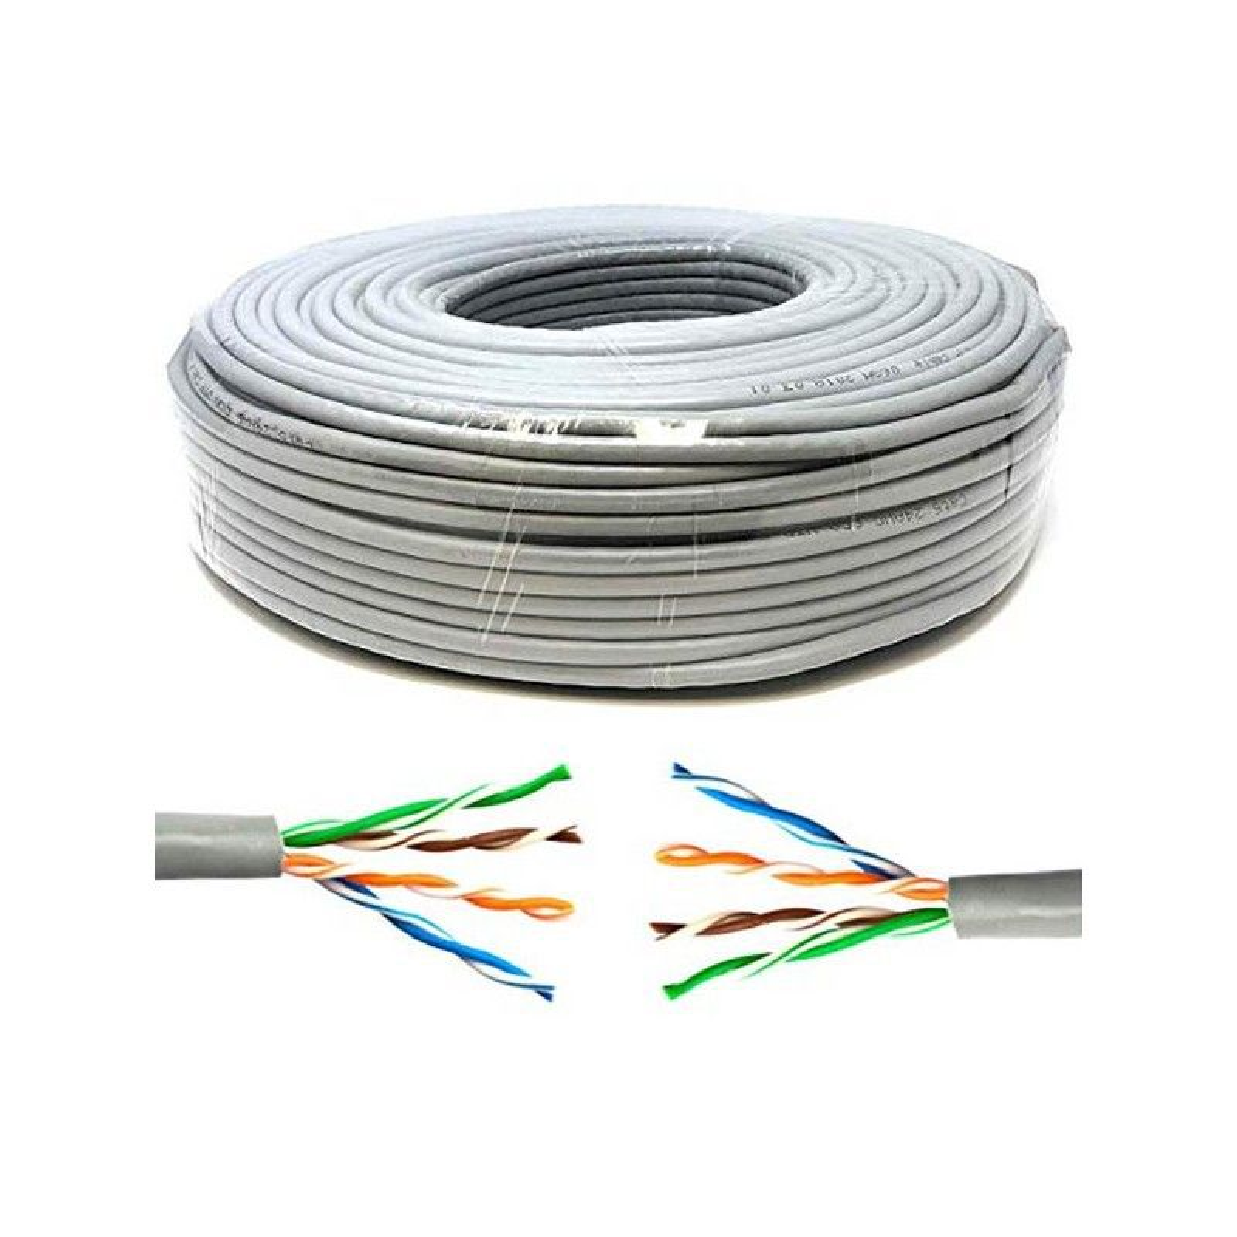
\includegraphics[width=.6\textwidth]{img/bobina_UTP.pdf}\footnote{Licencia Creative Commons by https://solarmat.es}
  \end{center}

Existen diferentes tipos de cables de datos: UTP, STP, FTP:
\begin{itemize}
\item Los cables \textbf{UTP} no disponen de protección ante interferencias electromagnéticas.
  \begin{center}
  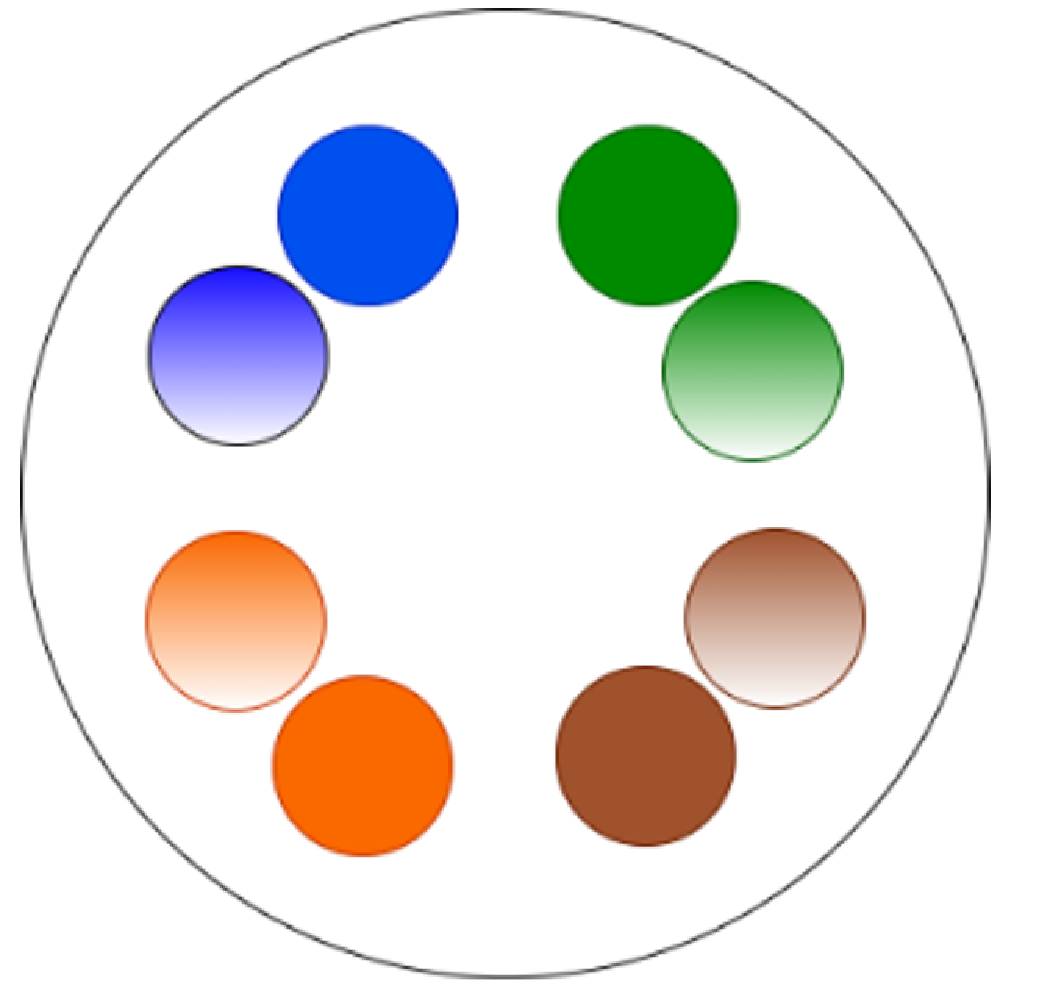
\includegraphics[width=0.4\textwidth]{img/UTP.pdf}
  \end{center}

\item Los cables \textbf{FTP} disponen de una pantalla global contra interferencias electromagnéticas dentro de la camisa de PVC que recoge los 4 pares destinados a transmisión de datos.
  \begin{center}
  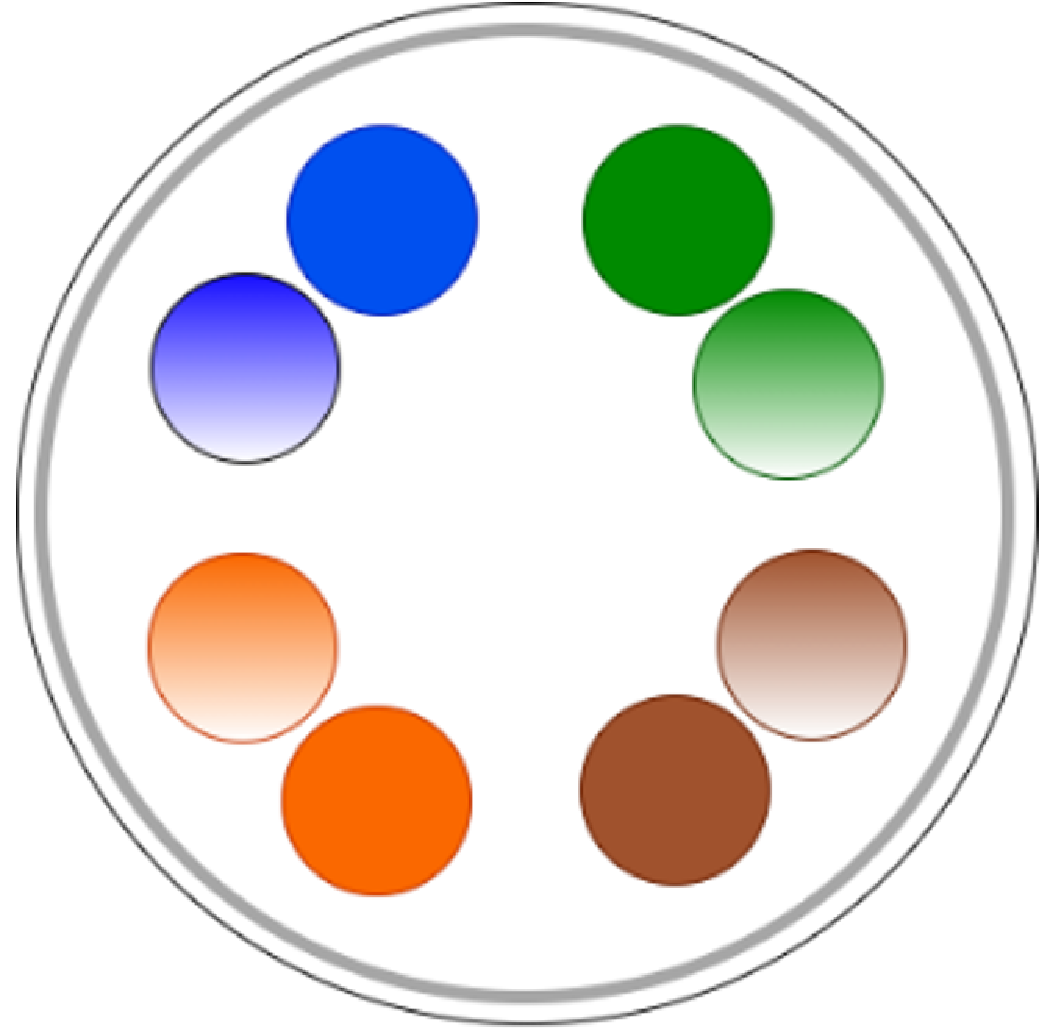
\includegraphics[width=0.4\textwidth]{img/FTP.pdf}
  \end{center}

\item Los cables \textbf{STP} disponen de una pantalla contra interferencias electromagnéticas por cada par de cables pero, además, también cuentan con una malla metálica exterior.
  \begin{center}
  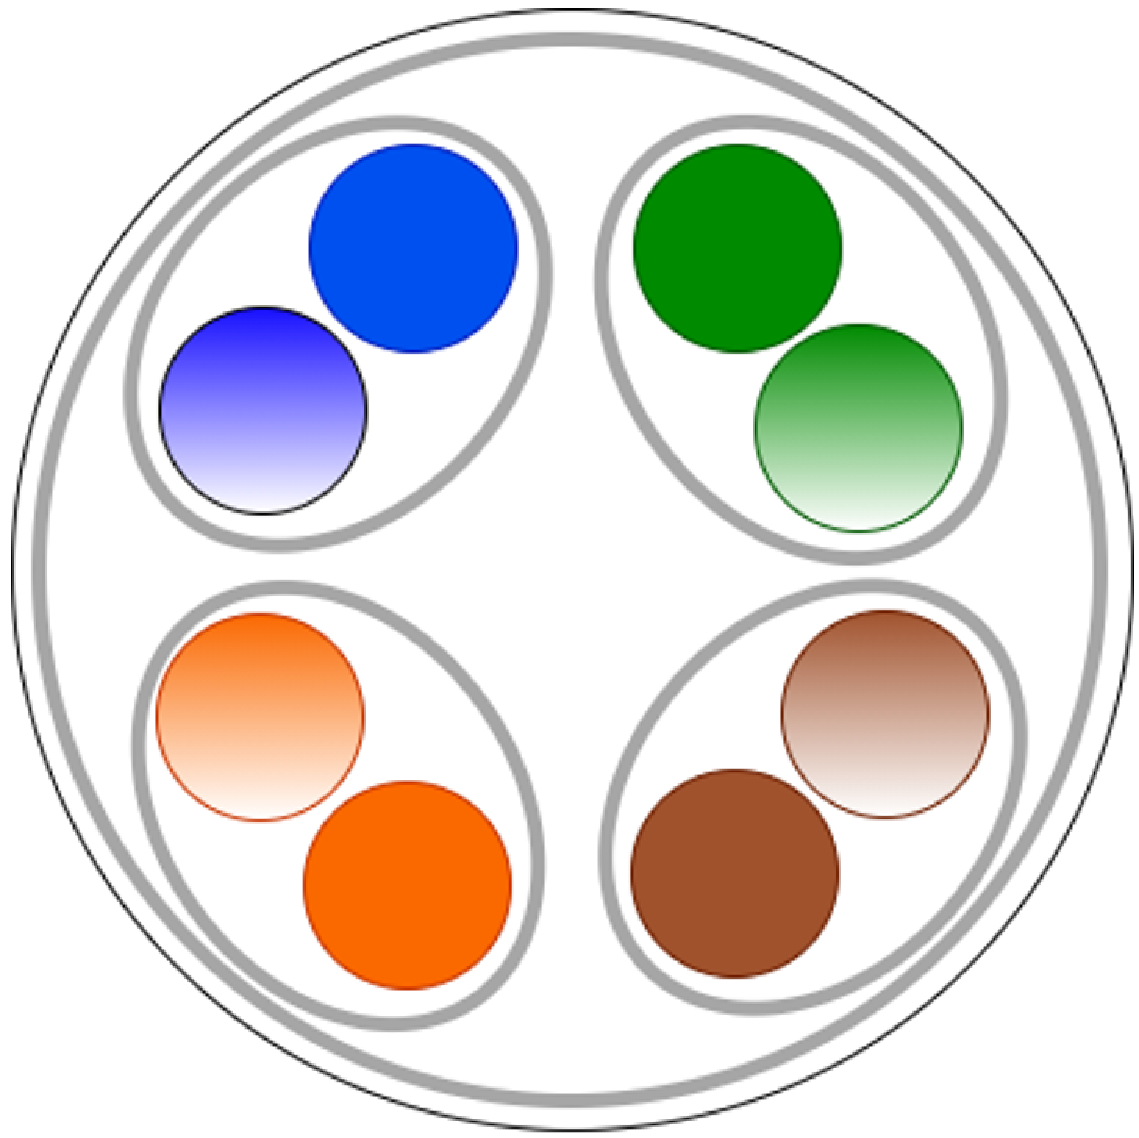
\includegraphics[width=0.4\textwidth]{img/STP.pdf}
  \end{center}

\emphEn nuestro caso utilizaremos UTP puesto que no necesitamos un apantallamiento ya que no transmitiremos datos y tampoco tendremos un alto grado de interferencias.

\section{Placa de Pruebas o ProtoBoard}
Es un tablero electrónico para realizar pruebas. Protoboard es la agrupación de los términos ingleses “prototype board”.
Esta protoboard la he instalado para poder hacer fácilmente el interconexionado entre los cables que llegan de los relés y los que van a la Raspberry Pi, evitando posibles tirones y movimiento de cables a la hora de hacer alguna manipulación.
Éstas, disponen de tres zonas diferenciadas:

\begin{itemize}
    \item \textbf{Canal Central}: Está situada en el medio de la placa y es donde se colocan los circuitos.
    \item \textbf{Buses}: Se sitúan en los extremos de la placa y disponen de dos líneas:
    \item \textbf{Línea roja}: Bus positivo o de voltaje.
    \item \textbf{Línea azul}: Bus negativo o de tierra.
    \item \textbf{Pistas}: Se sitúan en la zona central de la placa y, conducen en sentido contrario de las líneas rojas y azul.
\end{itemize}

\begin{center}
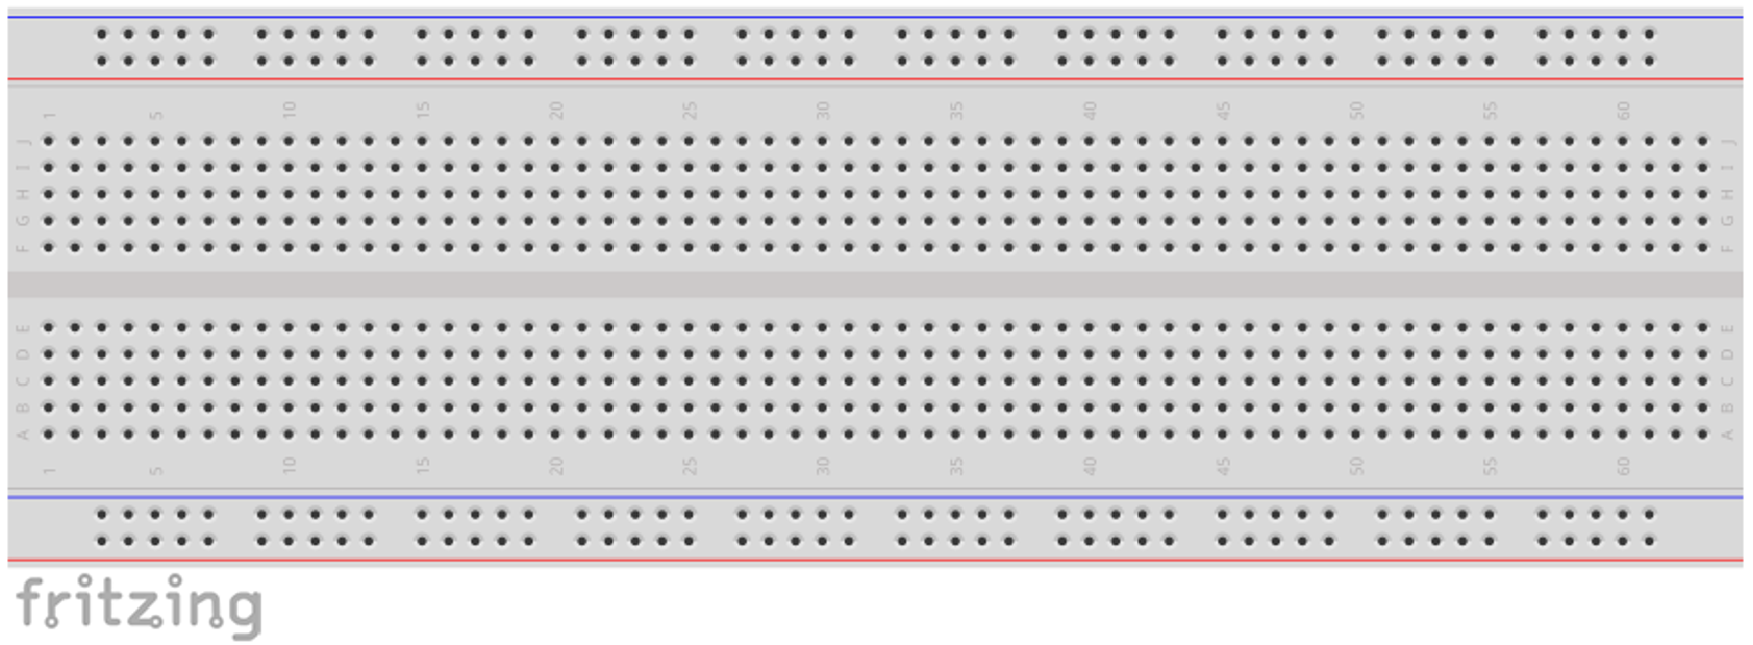
\includegraphics[width=0.9\textwidth]{img/protoboard.pdf}
\end{center}

\section{Router}
Es un dispositivo que nos permite interconectar diferentes redes de datos. En mi caso dispongo de un router con WiFi integrado para poder dotar a la Raspberry Pi de salida a Internet.
Al principio, estuve valorando la opción de ‘tirar’ un cable de datos desde la primera caja de derivación después del Cuadro General de Mando y Protección o Cuadro eléctrico, hasta el RTR (Registro Terminación de Red) que es donde tengo la línea de datos más cercana, pero en único tubo que comunica es de naturaleza eléctrica y no está bien mezclar tipos de instalaciones.

Adjunto un pequeño dibujo informativo para que se pueda entender la instalación:
\begin{center}
\includegraphics[width=0.9\textwidth]{img/Diagrama Básico.pdf}
\end{center}


\end{itemize}

